\documentclass[12pt,a4paper]{report}
\usepackage[utf8]{inputenc}
\usepackage{amsmath}
\usepackage{amsfonts}
\usepackage{amssymb}
\usepackage{graphicx}
\usepackage{float}
\usepackage{color}
\author{Malcolm Watt}
\title{Numerical Methods Assignment 2}
\usepackage{sectsty}
\begin{document}

\maketitle
\section*{Chaper 3 Exercises}
\subsection*{Question 3.3}
The linear least squares system is given as follows:
{\color{blue}
$$A x= 
\begin{bmatrix}
1 & e\\
2 & e^2\\
3 & e^3
\end{bmatrix}
\begin{bmatrix}
x_1 \\ x_2
\end{bmatrix}
\approx
\begin{bmatrix}
2 \\
3 \\
5
\end{bmatrix}
= b
$$
}
\subsection*{Question 3.18}
Consider the vector $$ a = \begin{bmatrix}2\\3\\4\end{bmatrix}$$.
\subsubsection{(a)}
We need to annihilate the third component of a, using an elementary elimination
matrix. The easiest is to subtract twict the first column from the last column.
Therefore the elementary row elimination matrix is given as
{\color{blue}
$$\begin{bmatrix}
1 & 0 & 0\\
0 & 1 & 0\\
-2 & 0 & 1\\
\end{bmatrix}$$
}
\subsubsection{(b)}
Now we need to do the same thing but with a Householder transformation.
We want to apply two Householder transformations, the first $H_1$ eliminating all
but the first element, and the second $H_2$ eliminating all but the second element.
Then it stand that the Householder matrix $H$ which eliminates only the third
element is simply the matrix multiplication of $H = H_1H_2$.

Let's find $H_1$
$$
v = a - \alpha (e_1) =
\begin{bmatrix}
2\\
3\\
4
\end{bmatrix}
- \alpha
\begin{bmatrix}
1\\
0\\
0
\end{bmatrix}
$$
where $\alpha = \pm \lvert \lvert a \rvert \rvert_2 = \pm \sqrt{29}$. Since $a_1$ is positive, we should use the negative $\alpha$ to avoid cancellation.


Following this we have
$$
v = a - \sqrt{29}
\begin{bmatrix}
1\\
0\\
0
\end{bmatrix}
=
\begin{bmatrix}
2 - \sqrt{29}\\
3\\
4
\end{bmatrix}
$$

and Householder matrix

$$H_1 = I - 2\frac{vv^T}{v^Tv} = 
\begin{bmatrix}
0.6885828  & 0.37139068& -0.62283441\\
0.37139068 & 0.55708601 & 0.74278135\\
-0.62283441 & 0.74278135& -0.24566881
\end{bmatrix}
$$

by a similar process we find 
$$
H_2 =
\begin{bmatrix}
  1.45796221 & 0.64642473&-1.19938586\\
 0.64642473 & 1.22908525 & 1.43036648\\
-1.19938586 & 1.43036648 &-0.68704746
\end{bmatrix}
$$

and the desired 

{\color{blue}
$$H = H_1 + H_2 = 
\begin{bmatrix}
 1.37716559  &0.74278135& -1.24566881\\
  0.74278135  &1.11417203 & 1.48556271\\
 -1.24566881  &1.48556271 &-0.49133762
\end{bmatrix}
$$
}
\subsubsection{(c)}
We pick the Given's Rotation matrix such that G is of the form
$$
\begin{bmatrix}
1 & 0 & 0\\
0 & c & s\\
0 & -s & c
\end{bmatrix}
$$

Since $\lvert a_3 \rvert > \lvert a_2 \rvert$ we use the cotangent formulation
to find $c$ and $s$. We have $\tau = c / s = \frac{a_3}{a_2} = 0.75$ and
therefore
$$s = \frac{1}{\sqrt{1+ \tau^2}} =\frac{4}{5}$$
and
$$c = \frac{3}{5}.$$

so the givens rotation matrix is

{\color{blue}
$$G = \begin{bmatrix}
1&0&0\\
0&\frac{3}{5}&\frac{4}{5}\\
0&\frac{-4}{5}&\frac{3}{5}
\end{bmatrix}
$$
}

\subsection*{Question 3.24}
Alright, well the obvious first step is to figure
out what is the QR factorization by Householder...

We expect an $m*n$ matrix to have dominant term
$n^2m-\frac{n^3}{3}$.

Let's go down the diagonal:
The selection of $v_i$ for the $i^{th}$ diagonal
term requires the calculation of the 2-norm.
Starting at the $i^{th}$ position this requires
$m-i$ multiplications, one square root (which
has the same complexity as a division) and 1
addition (that is the norm vector plus the column
we are annihilating).

The algorithm requires
$$\sum_{k=1}^{n}(2(m-k)+\sum_{j=k}^{n}2(m-k))
=\sum_{k=1}^{n}(2(m-k)+2(m-k)(n-k))$$
$$=\sum_{k=1}^{n}2(mn+m)n-(m+n+1)n(n+1) +
n(n+1)(2n+1)/3$$

from which the dominant term is $mn^2-n^3/3$
multiply-add operations.

{\color{red}
\subsection*{Question 3.25}
}
\section*{Chapter 3 Programming Questions}
\subsection*{Question 3.1}
The code for this question can be found in
assignment2.ipynb.

The results are shown in the following figure for different orders of polynomials. Which polynomial
fits this the best is the question. Now, if there
is absolutely no error, and we know these are
the correct points, then the order 5 polynomial
is the best fit. Obviously the 0 order polynomial
is basically garbage. If we know the data is
relatively noisy, then we'll want to pick one
of the least aggressive approximations (i.e. the
linear fit). Really it depends on the data what
the actual correct answer is, the key thing to
keep in mind is that the higher the order
of the polynomial, the more it will fit to the
particular examples given, and perhaps not
generalize well to a noisier set of results
that are not included in this "training set".

\begin{center}
\begin{figure}[H]
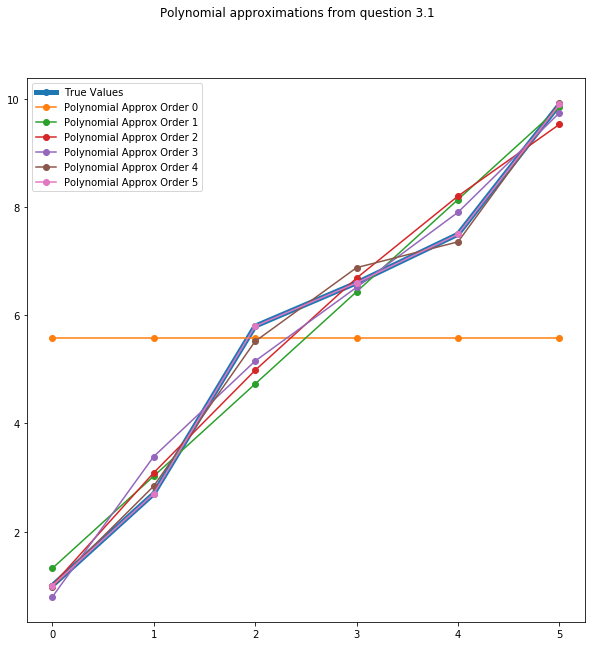
\includegraphics[width=\textwidth]{poly_approx.png} 
\end{figure}
\end{center}

\subsection*{Question 3.3}
The results and discussion can be found in the ipython notebook.


\subsection*{Question 3.4}
The results and discussion can be found in the
ipython notebook.

\subsection*{Question 3.5}
The results and discussion can be found in the
ipython notebook.


\section*{Chapter 4 Exercises}
\subsection*{Question 4.3}
Find the eigenvalues and corresponding eigenvectors for the following matrix:
$$A = \left( \begin{smallmatrix}
1&2&-4\\
0&2&1\\
0&0&3
\end{smallmatrix} \right)
$$

$$A - \lambda I = 0 $$
$$\left( \begin{smallmatrix}
1-\lambda&2&-4\\
0&2-\lambda&1\\
0&0&3-\lambda
\end{smallmatrix} \right) X = 0
$$

$$
det(\left( \begin{smallmatrix}
1-\lambda&2&-4\\
0&2-\lambda&1\\
0&0&3-\lambda
\end{smallmatrix} \right) ) = -\lambda^3 + 6 \lambda^2 - 11 \lambda + 6 = -(\lambda - 1)(\lambda -2)(\lambda -3)
$$

Which has roots at $\lambda = 3, \lambda = 2, \lambda = 1$.
The corresponding eigenvectors are
for $\lambda = 1 \rightarrow \left(\begin{smallmatrix}1\\0\\0\end{smallmatrix}\right)$,
for $\lambda = 2 \rightarrow \left(\begin{smallmatrix}2\\1\\0\end{smallmatrix}\right)$,
for $\lambda = 3 \rightarrow \left(\begin{smallmatrix}-1\\1\\1\end{smallmatrix}\right)$.


\subsection*{Question 4.9}
PART A


Let $Ax = \lambda x$.
$$\lambda \bar{x}^T x = \bar{x}^T(\lambda x)$$
$$= \bar{x}^T A x$$
$$=(A^T \bar{x})^Tx$$
$$=(A \bar{x})^Tx$$
$$=(\bar{A}\bar{x})^T x$$
$$=(\bar{\lambda}\bar{x})^T x$$
$$=\bar{\lambda}\bar{x}^Tx$$

Since $x \neq 0$, $\bar{x}^Tx \neq 0$ and $\lambda = \bar{\lambda}$ which means $\lambda$ is real.


PART B
Again, we have $Ax = \lambda x$.

Multiplying by $x^H$, that is $\bar{x}^T$, from the left, we get

$$x^H(Ax) = x^H(\lambda x)$$
$$ = \lambda x^H x$$
$$ = \lambda \lvert \lvert x \rvert \rvert.$$


Now if we take the Hermitian of both sides:
$$x^H A^H x = \bar{\lambda} \lvert \lvert x \rvert \rvert.$$

Since A is a Hermitian matrix, we have $A^H = A$, so then the lhs becomes

$$x^H A^H x = x^H A x$$
$$= x^H \lambda x$$
$$ = \lambda \lvert \lvert x \rvert \rvert.$$

and we then obtain
$$\lambda \lvert \lvert x \rvert \rvert = \bar{\lambda} \lvert \lvert x \rvert \rvert.$$
Since x is an eigenvector, it is by definition not the zero vector and so the length
of the vector is not zero. If we divide both sides of the above equation by the length
(we don't have to worry about division by zero), we get $$\lambda = \bar{\lambda}$$
therefore $\lambda$ is a real number.

Since $\lambda$ is any eigenvalue, we can conclude that for all eigenvalues of a hermitian
matrix A, we have real valued eigenvalues.

\subsection*{Question 4.10}
This can be proven by counter-argument.
If the eigenvalue is to be positive, it can not be negative or 0.

Let's consider the case where the eigenvalue is 0. If $\lambda=0$,
then there must exist an eigenvector $x$ so that $Ax = 0$, however, if we have
$Ax=0$, then $x^TAx = 0$, so A is not positive definite.

Now let's consider the case where the eigenvalue is negative. If we have
$\lambda < 0$, then there is some eigenvector $x$ so that $Ax = \lambda x$,
which then means we have $x^TAx=\lambda \lvert x \rvert^2$. Since we have a
negative eigenvalue, and the squared eigenvector is positive, we necessarily
have a negative right hand side, and so the matrix A does not satisfy the
condition for being positive definite.

Therefore, if a matrix A is positive definite, it necessarily has positive eigenvalues.

\subsection*{Question 4.15}
In order for A to be invertible in the first place, we need the eigenvalues of A to be
non-zero. So with

$$Ax = \lambda x$$
we can multiply by $A^{-1}$ from the left to get

$$A^{-1}Ax = \lambda A^{-1}x$$
$$x= \lambda A^{-1}x$$
and rearranging it to look more like the standard eigenvalue equality we then have
$$A^{-1}x = \frac{1}{\lambda}x$$
so all eigenvalues of a non-singular matrix A are the reciprocal of corresponding
eigenvalues for the inverse matrix $A^{-1}$.

Note that this equality has not changed the x in the eigenvalue equation,
therefore for each eigenvalue $\lambda$ and eigenvector $x$ of A, we have a corresponding
eigenvalue $\frac{1}{\lambda}$ and unchanged eigenvector $x$ for $A^{-1}$.

\subsection*{Question 4.19}

\subsection*{Question 4.25}


\section*{Chapter 4 Programming Problems}
\subsection*{Question 4.2}
The results and discussion can be found in the ipython notebook.

\subsection*{Question 4.5}
The results and discussion can be found in the ipython notebook.

\subsection*{Question 4.7}
The results and discussion can be found in the ipython notebook.

\subsection*{Question 4.9}
The results and discussion can be found in the ipython notebook.

\subsection*{Question 4.15}
The results and discussion can be found in the ipython notebook.


\end{document}